%% This is file `elsarticle-template-1-num.tex',
%%
%% Copyright 2009 Elsevier Ltd
%%
%% This file is part of the 'Elsarticle Bundle'.
%% ---------------------------------------------
%%
%% It may be distributed under the conditions of the LaTeX Project Public
%% License, either version 1.2 of this license or (at your option) any
%% later version.  The latest version of this license is in
%%    http://www.latex-project.org/lppl.txt
%% and version 1.2 or later is part of all distributions of LaTeX
%% version 1999/12/01 or later.
%%
%% Template article for Elsevier's document class `elsarticle'
%% with numbered style bibliographic references
%%
%% $Id: elsarticle-template-1-num.tex 149 2009-10-08 05:01:15Z rishi $
%% $URL: http://lenova.river-valley.com/svn/elsbst/trunk/elsarticle-template-1-num.tex $
%%
% \documentclass[preprint,12pt]{elsarticle}

%% Use the option review to obtain double line spacing
\documentclass[preprint,review,12pt]{elsarticle}

%% Use the options 1p,twocolumn; 3p; 3p,twocolumn; 5p; or 5p,twocolumn
%% for a journal layout:
%% \documentclass[final,1p,times]{elsarticle}
%% \documentclass[final,1p,times,twocolumn]{elsarticle}
%% \documentclass[final,3p,times]{elsarticle}
%% \documentclass[final,3p,times,twocolumn]{elsarticle}
%% \documentclass[final,5p,times]{elsarticle}
%% \documentclass[final,5p,times,twocolumn]{elsarticle}

%% The graphicx package provides the includegraphics command.
\usepackage{graphicx}
\usepackage{caption}
\usepackage{subcaption}

%% The amssymb package provides various useful mathematical symbols
\usepackage{amssymb}
%% The amsthm package provides extended theorem environments
%% \usepackage{amsthm}

%% The lineno packages adds line numbers. Start line numbering with
%% \begin{linenumbers}, end it with \end{linenumbers}. Or switch it on
%% for the whole article with \linenumbers after \end{frontmatter}.
% \usepackage{lineno}

%% natbib.sty is loaded by default. However, natbib options can be
%% provided with \biboptions{...} command. Following options are
%% valid:

%%   round  -  round parentheses are used (default)
%%   square -  square brackets are used   [option]
%%   curly  -  curly braces are used      {option}
%%   angle  -  angle brackets are used    <option>
%%   semicolon  -  multiple citations separated by semi-colon
%%   colon  - same as semicolon, an earlier confusion
%%   comma  -  separated by comma
%%   numbers-  selects numerical citations
%%   super  -  numerical citations as superscripts
%%   sort   -  sorts multiple citations according to order in ref. list
%%   sort&compress   -  like sort, but also compresses numerical citations
%%   compress - compresses without sorting
%%
%% \biboptions{comma,round}

% \biboptions{}

\journal{Professor Torsten Suel}

\begin{document}

\begin{frontmatter}

%% Title, authors and addresses

\title{Wikipedia Reputation System Based on Edit History}

%% use the tnoteref command within \title for footnotes;
%% use the tnotetext command for the associated footnote;
%% use the fnref command within \author or \address for footnotes;
%% use the fntext command for the associated footnote;
%% use the corref command within \author for corresponding author footnotes;
%% use the cortext command for the associated footnote;
%% use the ead command for the email address,
%% and the form \ead[url] for the home page:
%%
%% \title{Title\tnoteref{label1}}
%% \tnotetext[label1]{}
%% \author{Name\corref{cor1}\fnref{label2}}
%% \ead{email address}
%% \ead[url]{home page}
%% \fntext[label2]{}
%% \cortext[cor1]{}
%% \address{Address\fnref{label3}}
%% \fntext[label3]{}


%% use optional labels to link authors explicitly to addresses:
%% \author[label1,label2]{<author name>}
%% \address[label1]{<address>}
%% \address[label2]{<address>}

\author[label1]{Heng Lin}
\author[label2]{Liang Niu}
\address[label1]{hl2521@nyu.edu}
\address[label2]{ln932@nyu.edu}

\begin{abstract}
%% Text of abstract
  We will present a reputation system for the well know Wikipedia website based
  on the edit history of their articles. In our system, editors will gain
  reputation score from their edit(contribution) to some particular article,
  they may also lose their score if they did some bad editting behavior like
  vandalism\cite{adler2007content}. Our model is based on the previous work of Adler and
  Alfaro \cite{adler2007content} , in their model they didn't consider the
  absolute time for edit survival, we improved their model by adding factors
  generated from editing frequency calculated using absolute time.
  We have implemented a system to calculate the reputation score for all authors
  in an article for Wikipedia, and we also evaluate our model by visualing the
  reputation score for every word's author and compare it to the evaluation
  system in Wikipedia.
\end{abstract}

\begin{keyword}
Wikipedia \sep reputation system \sep Edit History
%% keywords here, in the form: keyword \sep keyword

%% MSC codes here, in the form: \MSC code \sep code
%% or \MSC[2008] code \sep code (2000 is the default)

\end{keyword}

\end{frontmatter}

%% main text
\section{Introduction}
\subsection{Basic Concepts in Wikipedia}
Wikipedia is a free online encyclopedia that aims to allow anyone to edit any
article and create them. Wikipedia is the largest and most popular general
reference work on the Internet and is ranked among the ten most popular
websites. Wikipedia is owned by the nonprofit Wikimedia
Foundation.\cite{wiki:wiki} Wikipedia is basically a set of articles that can be
editted by anyone. Anonymous user can also be able to edit any articles without
registration, though Wikipedia do provide registration function.
Thus it will
cause some problems. For example, some
articles will be editted by users maliciously. They may want to damage some
articles or introduce bias or mistakes into some particular articles for their
own interest. This kind of behavior is also called ``Vandalism''
\cite{wiki:vandalism}. Vandalism is very common in Wikipedia, thus there is a
terminology ``Edit War''\cite{wiki:edit_war} to describe the circumstance when
serval people are trying to take control of an article. In our model, we tried
to build a reputation system for Wikipedia so that we can generate reputation
score for every author of an article, by doing that, we can decide to trust high
reputation authors more because they have proved that they can do good editting.
\subsection{Reputation System}
As we said above, the system we want to build is a reputation system for
authors. To achieve this goal, what we are doing is to generate a score for
every edit. It is easy to check all edit history of a single article in
Wikipedia. By fetching the edit history data, we actually get all revision from
the very beginning of the article to some particular time point. In our
experiment, we used a crawler to fetch such data so we can have latest version
of an article. The data in stored in the manner that every edit is a full
article. It is stored not the patches between two versions but full version for
every edit. \\
For every edit, or for every revision, our model is to consider the edits around
it. By saying some edits is ``around'' a edit, we are actually saying that
all revisions are sorted in time sequence, and some edits are closed to a edit
either they are n-neighbors (in particular, we take n equals to 3 or 10) of this
edit or they have short time gap with this edit (in our model, we take this time
gap as 1hr).
\subsection{Applications}
Reputation system can play a significant role in building a healthy wiki
community, because it promotes the quality of articles in many ways. If editors
can view previous editting history and their authors' reputation, they can
decide whether to keep the edit or not more easily. If we compare the Wikipedia
community, which is a knowledge contributing community, to Github, which is a
code contributing community, then those who have high reputation are like
programmers who have many stars and followers. High reputation will make an
author looks more reliable and help other authors make decisions.\\
Besides, we can visulize the reputation distribution of an article. through that
way, it will be obvious that what kinds of article will attract more high
reputation authors and based on that, it will be intriguing to discuss the
relationship between articles' topic and their authors. We tried to do that a
little bit, even not fully discovered. And another way to use reputation is to
reward those high reputation authors to promote their passion. Also reputation
score itself is some kind of honor on the Internet.


% template for inserting pictures
% \begin{figure}[h]
% \centering\includegraphics[width=0.4\linewidth]{figure}
% \caption{Figure caption}
% \end{figure}

\section{Related Work}
% adlar, zeng, 2008 length->quality, assign trust
The work most related to ours is \cite{adler2007content}, where Wikipedia
revisions are used to evaluate authors' reputation. Our work is mostly based on
theirs and then do some change or improvement. Also, to discuss the relationship
between reputation and article quality is inspired by Aniket Kittur's work done
in 2008 \cite{kittur2008can}, in which they use Amazon's crowdsourcing service
called ``Amazon Mechanical Turk'' to evalute the quality of a Wikipedia article.
They found that people tend to give higher score to those articles that have
more high reputation authors. This leads us to use quality of an article as a
evalutation metrics. To evaluate article's quality, we found that Joshua E.
Blumenstock's work \cite{blumenstock2008size} is a quite intuitive way.
Actually, at the early stage of our thinking, we have considered using word
length as an important factor to evaluate edit quality. Zeng's work
\cite{zeng2006computing} is one of the most successful work done in 2000s, in
which they used dynamic Bayesian Network to evaluate quality or trust for an edit. We
took a quick look on it but the Bayesian Network method is not we are looking
for, we hope to find a way that use edit history more directly to reflect how
good a revision is. In many edit history based systems, like adlar's work
\cite{adler2007content} and Wohner's work \cite{wohner2009assessing}, editting
distance is used to evaluate difference between two versions. And we got the
idea of coloring text as visulization from adler's work
\cite{adler2008assigning}, in which they assigned text color to compare
difference between two revisions. We use coloring in a different way, we assign
words colors according to their authors' reputation to see an article's authors'
distribution, which will be explained later.

\section{Reputation Model}
\subsection{Notation}
We use the similar notation in Adler \cite{adler2007content}. The following is
the notations we are using:\\
For some particular article, let's say the Wikipedia entry ``Reverse
Engineering'', there are many versions of it.
For all the versions, we sorted them in a time sequence, and thus there are
versions from very beginning to latest. We call these versions $v_0, v_1, v_2$
and so on. And we assume $v_0$ is empty, which means we divide the creating of
an article into two versions, one is $v_0$, the empty article, one is $v_1$, the
first version with content. In most cases, the creator of an article will give
some content to it, so we are actually adding an empty version before the first
version. And thus we introduce the concept revision:\\
\subsubsection{Adler's notation}
we use $r_i$ means the $i_{th}$ edit of an article, which is used to refer to
the change from $v_{i-1} to v_i$.\\
$d$ edit distance, not like traditional editting distance calculation, we will
measure edit distance based on words, somehow like the tool ``diff''.\\
$a_i$ is the author of $v_i$. Because there may be continuous edits done by the
same author, we will eliminate this situation by merging a few continuous edit
done by same author to one edit, or keep only one with others deleted. One thing
that is different from Adler's is that in our improvement, we considered
anonymous user(even though they are anonymous, we can get their IP address
through Wikipedia's API) as useful users. So this notation has different meaning
in Adler's model and our model. Adler exclude anonymous authors' contribution,
but we consider them as registered users.\\
$txt(i,j)$, in which $0 < i \leq j \leq n$. This is the notation to note how
many words that are introduced in the edit of $v_i$ are still left in $v_j$.\\
If $i = j$, then this means the amount of words that added to this article in
$r_j$. All the amount is measured by number of words.\\
$d(v_i,v_j)$, in which $0 < i \leq j \leq n$. It is edit distance between $v_i$
and $v_j$. When $i=j$, of course it equals to 0.\\
\subsubsection{Our own notation}
And the following notations is for our improvement of Adler's model. Cause we
take absolute time into account, we define that:\\
$t(r_i)$, is the timestamp of edit $r_i:from r_{i-1} to r_i$.\\
And also $g(r_i)$, the average edit time gap for some edit $r_i$. It is computed
by the following process:\\
For some edit $r_i$, find all the edit histories that happened in $[
  t(r_i)-30min, t(r_i)+30min]$, say there are $n$ edit between this time gap.
Then $g(r_i) = \frac{60min}{n}$. This notation is related with the edit
frequency around some edit. Exeptions: for first a few edits and last a few
edits, we use a different formula: $g(r_i) = \frac{t_l}{n}$ in which $t_l$ is
the longest time that we can trace to, for first a few edits, this time is
$30min+t(r_i)$, for last a few edits, this time is $30min+(t(r_k)-r(r_i))$, in
which $r_k$ is the newest edit.
\subsection{Concepts}
We introduce some concepts that is useful for our model.\\
First one is authorship. Authorship is defined as the authorship of a word. Say
an article ``Reverse Engineering'', there are about 800 authors. And we can
imagine that different words are writed by different users. There is an
algorithm that can show for a particular version of this article, who is the
author of which part. Say an article has 5 words: $w_0 to w_4$, and this
algorithm can show the authors for all these 5 words: $a_0 to a_4$. Authorship
is an important concept, we will use it in calculating $txt(i,j)$ and also in
our improvement. We will also show authorship of an article.\\

\subsection{Adler's Model}
% about how we reproduce adlar's model and give out experiments result for a
% single page
In this part we will simply introduce Adler's model of content-driven reputation
system in a versioned document and our implementation.\\
\subsubsection{Rule 1}
Basically, there are two rules in Adler's model, the first one is based on what
they called ``Text Survial''. It is the idea that if text introduced by $r_i$ is
still present in $v_j$, then this can indicate that the author of $v_j$ agrees
that $r_i$ is a good or valuable edit. Thus, they proposed their first rule:\\
\newtheorem{ruullee}{RULE}
\begin{ruullee}[(reputation update due to text survival)]
  When the revision $r_j$ occurs, for all $0<j<i$ such that $j-i \leq 10$ and
  $a_j \neq a_i$, we add to the reputation of $a_i$ the amount:\\
  \[
  \centering c_{scale}*c_{text}*\frac{txt(i,j)}{txt(i,i)}*(txt(i,i))^{c_{len}}*log(1+R(a_j,r_j))
  \]
  where $c_{scale} > 0, c_{text} \in [0,1]$, and $c_{len} \in [0,1]$ are
  parameters, and where $R(a_j, r_j)$ is the reputation of $a_j$ at the time
  $r_j$ is preformed. 
\end{ruullee}
\subsubsection{Rule 2}
The second rule is based on the idea of ``Edit Survival'', the rule is as
follows:\\
\begin{ruullee}[(reputation update due to edit survival)]
  When the revision $r_j$ occurs, for all $0<i<j$ such that $j-i \leq 3$, we add
  to the reputation of $a_i$ an amount q determined as follows. If $a_j=a_i$or
  $d(v_{i-1}, v_i)=0$, then $q=0$; otherwise, q is determined by the following
  algorithm.
  \[
    \centering
    q := \frac{c_{slack}*d(v_{i-1},v_j) - d(v_i,v_j)}{d(v_{i-1},v_i)}
  \]
       if $q<0$ then $q:=q*c_{punish}$ endif
  \[
    \centering
    q := q*c_{scale}*(1-c_{text})*(d(v_{i-1}, v_i))^{c_{len}}*log(1+R(a_j,r_j))
  \]
\end{ruullee}
Basic idea behind this rule is that using edit distance to trace how much left
for a edit in next 3 edits. The more left, the more reputation should be given
to the author.

\subsubsection{Implementation}
When we are implementing this model, we are using Google's library called
``diff\_match\_patch'' to help us do the edit distance calculation, which is
based on the algorithm described in Myers' work \cite{myers1986ano}.\\
We also discovered some details in his model. What he didn't mentioned is that
authorship 


\subsection{Our Improvement}
\subsubsection{Take Timestamp into Account}
% about asuumption of authors' passion, how we introduce time stamp as a factor,
% and how to adjust model, and why we do this and the benefit and give out result.
% AAAnd also, we take IP into account.
\subsubsection{Take Anonymous Users into Account}

\begin{figure}[h]
  \centering

    \begin{subfigure}{0.5\textwidth}
    \centering 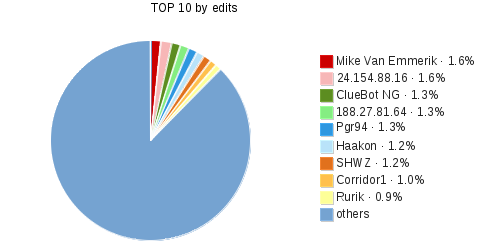
\includegraphics[width=0.9\linewidth]{pic/wiki1.png}
    \caption{TOP 10 by edits}
    \label{fig:wiki1}
    \end{subfigure}

    \begin{subfigure}{0.5\textwidth}
    \centering 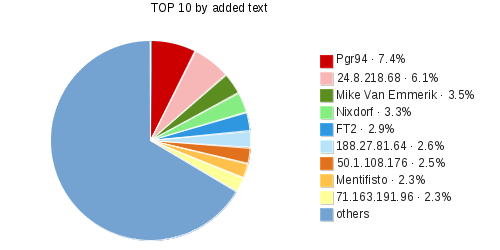
\includegraphics[width=0.9\linewidth]{pic/wiki2.png}
    \caption{TOP 10 by added text}% ``Reverse Engineering''}
    \label{fig:wiki1}
    \end{subfigure}

  \caption{TOP 10 by two metrics of ``Reverse Engineering''}
\end{figure}


\subsection{Edit War Optimization}

\section{Authorship}
% authorship defination, usage, algrithm introduction, why we use it.

\subsection{Authorship as Evaluation}
% talk about authorship and visulization, and based on visulization discuss our
% result and the original model's result. 

\subsection{Authorship and Article Quality}

\subsection{Conclusion}

\section{Self Assessment}

%% The Appendices part is started with the command \appendix;
%% appendix sections are then done as normal sections
%% \appendix

%% \section{}
%% \label{}

%% References
%%
%% Following citation commands can be used in the body text:
%% Usage of \cite is as follows:
%%   \cite{key}          ==>>  [#]
%%   \cite[chap. 2]{key} ==>>  [#, chap. 2]
%%   \citet{key}         ==>>  Author [#]

%% References with bibTeX database:

% \bibliographystyle{model1-num-names}
\bibliographystyle{ieeetr}

% \newpage

\section{\refname}

\bibliography{sample}


\end{document}